% ----------------------------------
% Cap Diseño
% ----------------------------------
%	Incluye
%		Diseño de interfaces y prototipos
%	    
%
\documentclass[a4paper,oneside,11pt]{book}

\usepackage[spanish,activeacute]{babel}
\usepackage[utf8]{inputenc}
%\usepackage[T1]{fontenc}
\usepackage{tabulary}
\usepackage{graphicx}

\usepackage{float}

\setcounter{secnumdepth}{3}

\oddsidemargin=0.2cm
\headsep=1cm
\textheight=21cm
\textwidth=16cm

% Personalizamos la separación entre párrafos...
\parskip=6pt

% Personalizamos el identado en la primera línea del nuevo párrafo...
\parindent=10pt

\begin{document}
% cuerpo del documento
\title{Navegaci'on}
\author{Pablo Eduardo Ojeda Vasco}
\date{\today}



	\maketitle
%
% Capítulo Diseño de interfaz de usuario
%
\chapter{Diseño} % (fold)
	\label{sec:diseno}

	\section{Diseño de navegación} % (fold)
	\label{sec:navegacion}
	
	% section diseño_de_la_interfaz_de_usuario (end)
	\subsection{Introducción} % (fold)
		\label{sub:nav_introduccion}
	
		Una vez que la arquitectura de la \textit{webapp} ha sido establecida y se han identificado sus componentes (páginas, textos, etcétera), deben definirse las rutas de navegación que permitan a los usuarios acceder al contenido y a las funciones de la aplicación web. Para hacer esto nos centraremos en dos aspectos. Por un lado identificar la semántica de navegación para los distintos usuarios del sitio; por otro lado definir la mecánica (sintaxis) para efectuar la navegación.
		
		Según la semántica, cada actor puede usar la aplicación en forma algo diferente, por lo que tendrán distintos requerimientos de navegación. Respecto a la mecánica, encontramos varias posibilidades, como las barras de navegación horizontal, los enlaces individuales, etcétera.
		
		% subsection nav_introduccion (end)
	
	\subsection{Tipos de menús de Navegación} % (fold)
	\label{sub:nav_contenidos_y_navegacion}
		
	En lo que atañe a la mecánica de navegación (que podemos definir como menús de navegación), se dispone de varias opciones:
	\begin{itemize}
		\item \textbf{Vínculo de navegación individual.} Incluye vínculos basados en texto, iconos, botones e interruptores, así como metáforas gráficas. Deben elegirse vínculos que sean apropiados para el contenido y consistentes con la heurística que conduzca al diseño de una interfaz de alta calidad.
		\item \textbf{Barras de navegación horizontal.} Enlista las categorías principales de contenido o de funciones en una barra que contiene vínculos apropiados.
		\item \textbf{Columnas de navegación vertical.} Enlista las principales categorías de contenido o funciones. Similar a las barras de navegación horizontal.
		\item \textbf{Pestañas}. Metáfora que no es más que una variación de la barra o columna de navegación y representa categorías de contenido o funciones como pestañas que se seleccionan cuando se requiere un vínculo.
	\end{itemize} 

	\fbox{\parbox{16cm}{\textbf{Menús de navegación.} Los menús de navegación deben estar siempre visibles y ubicados en la misma posición durante toda la navegación de la página. El diseño de la interfaz debe ser también accesible. 

	El cambio del posicionamiento de los menús de navegación provoca la desorientación del usuario. 

	Evitar los enlaces a secciones de la propia web que abran nuevas ventanas del navegador ya que esto dificulta la navegación lineal. Intentar que todo el contenido quede integrado siempre dentro de la misma ventana en la que se navega.}}
	
	% subsection contenidos_y_navegacion (end)
		
	\subsection{Navegación rápida y lineal} % (fold)
	\label{sub:nav_navegacion_rapida_y_lineal}
	
		\textbf{Navegación lineal.} El diseño debe permitir al usuario informarle en cada momento donde está, cómo ha llegado a ese lugar y cómo puede volver al inicio, tanto al inicio de la sección en la que está navegando como al inicio de la web de donde partió. 

		Utilizar enlaces de Inicio, Atrás y Adelante para facilitar la navegación lineal. Es más fácil que el usuario descubra todo el contenido de la web si avanza de forma progresiva regresando con facilidad al punto de inicio que ofreciendo todas las posibilidades en la Página de Inicio.
		
		\textbf{Navegación rápida.} Evitar los tiempos de descarga demasiados largos. El usuario puede pensar que el enlace no funciona e insiste presionando repetidamente el enlace, o desistir. 
	% subsection navegacion_rapida_y_lineal (end)
	
	\subsection{Aspectos a tener en cuenta en el diseño de menús de navegación} % (fold)
	\label{sub:nav_diseno_de_menu_de_navegacion}
	
		En los menús o barras de navegación, colocamos símbolos o texto con sus correspondientes enlaces a los distintos contenidos de la \textit{webapp}, para que el usuario pueda fácilmente encontrar lo que está buscando.
		
		Del párrafo anterior se desprende que \textbf{el diseño de esta navegación debe cumplir dos requisitos claves: simplicidad y claridad.}
		 
		\paragraph{Clara} % (fold)
		\label{par:nav_clara}
			Cuando el usuario entra en la página web, siguiendo un esquema mental que ha aprendido de sus visitas a otras webs, buscará la barra de orientación (lateral, superior, inferior).
			La estructura de navegación debe poder ser fácilmente identificable como tal, en tan sólo unos segundos, y una vez localizada en la página, rápida de comprender y de utilizar.
		% paragraph clara (end).
		
		\paragraph{Simple} % (fold)
		\label{par:nav_simple}
			Un vistazo a esa estructura de navegación debe permitir al usuario hacerse una idea de lo que puede encontrar en el web, le ayuda a decidir si se queda o bien se marcha a buscar en otra página o si le conviene más empezar la visita por un determinado enlace u otro.
			
		% paragraph simple (end)Simple.
		
		\fbox{\parbox{16cm}{Cuanto más simple sea la estructura de navegación, más rápido y fácil será interpretarla y reconocer así las distintas alternativas que ofrece la \textit{webapp}.}}
		
		Siguiendo con la idea de claridad, los contenidos de la estructura de navegación, que serán habitualmente o texto o imágenes o símbolos, requerirán:
		\begin{itemize}
			\item El texto en los enlaces (la etiqueta), debe facilitar información suficiente e inequívoca de los contenidos que se encontrarán al hacer clic sobre él.
			\item No colocar expresiones extrañas o misteriosas, desconcertantes o difíciles de reconocer, o bien nombres propios de productos o servicios que el usuario no puede reconocer. Si esto ocurre, ese enlace no cumple su objetivo de orientar.
			\item Facilitar el trabajo de localización de contenidos rápidamente y tendrás más oportunidades de que encuentren lo que tú quieres que lean.
			\item En las etiquetas, a veces será contraproducente ser muy creativo. Los usuarios ya han aprendido el significado de \textit{Política de Privacidad, Site Map, Homepage, Sobre nosotros, contacto, etcétera}. 
			\item Los símbolos o iconos deben ser también fáciles de interpretar visualmente .
		\end{itemize}
		
		
		Más necesidades a tener en cuenta para la estructura de navegación:
		
		\begin{itemize}
			\item \textbf{Consistente.} Una vez el usuario ha \textit{aprendido} cómo usar el menú de navegación, ésta estructura ha de mantenerse de manera consistente en todas las páginas para facilitar la comodidad y velocidad para encontrar la información.
			La consistencia debe ser tanto en su localización en la página, colores, fuentes, etiquetas y para los distintos submenús que pueda ser necesario desplegar.
			\item  \textbf{Los contenidos de la barra de navegación deben ser adecuados al comportamiento que anticipemos del usuario.}	Puesto que pretendemos conocer al usuario que usará la \textit{webapp}, se anticiparán sus necesidades de información y la respuesta a las preguntas más habituales que le surgirán, para decidir que enlaces van a ser incluidos en el menú de navegación y qué nombre le daremos.
			También el orden de los contenidos debe intentar seguir una lógica para el usuario, según las páginas de mayor interés o una agrupación coherente de los enlaces del web.
			\item \textbf{Ayudar al usuario.} Es importante que el usuario pueda distinguir qué símbolos tienen un enlace y los que no, para ahorrarle el tiempo de irlos probando.
			Hay que estudiar la profundidad de enlaces que se incluirán en la barra de navegación, a veces será bueno incluir distintos niveles de carpetas o directorios que despliegan más enlaces sucesivamente pero también será importante mantener la claridad y así no intentar mostrar todo en el menú, no sea que tantas opciones despisten al hacer al usuario dudar en su decisión rápida de dónde hacer click. Incluir siempre un enlace a la página principal, y un menú de navegación lineal por si el usuario se encuentra desorientado o en páginas muy profundas en la estructura y desea regresar a niveles superiores.
			Al ayudar al usuario a orientarse no sólo optimizas su tiempo sino que le puedes dirigir a aquellas páginas que te interese que vea.
		\end{itemize}
		
	
	% subsection diseño_de_barras_de_menú_de_navegación (end)
	
	\subsection{Diseño de menús de navegación} % (fold)
	\label{sub:nav_diseno_de_menus_de_navegacion}

		Una vez explicados los aspectos que se tendrán en cuenta en el diseño de navegación, como la simplicidad, la claridad, la consistencia, etcétera, el siguiente paso es realizar el diseño de los diversos menús de navegación.
		
		Para hacer esto, en primer lugar se explicarán los menús relacionados con el médico, a continuación los del paciente, los del administrador, los de las fichas médicas y por último con los de la página principal y todos aquellos para los que no es necesario estar registrado.
		
		\fbox{\parbox{15cm}{Merece la pena hacer resaltar que, al estar la aplicación desarrollada en dos idiomas, todos los menús de navegación estarán habilitados en el que indique el propio usuario.}}
		
	
		\paragraph{Menús de navegación de los médicos.} % (fold)
		\label{par:nav_menus_de_navegacion_de_los_medicos}
		
			En términos generales, en todas las pantallas del médico encontramos dos barras de navegación horizontales situadas siempre en la parte superior, una columna de navegación vertical (por cada sección) situada siempre en el extremo izquierdo y una barra de navegación rápida situada en la zona superior izquierda. Además, en diversas secciones aparecen vínculos de navegación individuales.
			
			\begin{figure}[H]
			  \centering
			    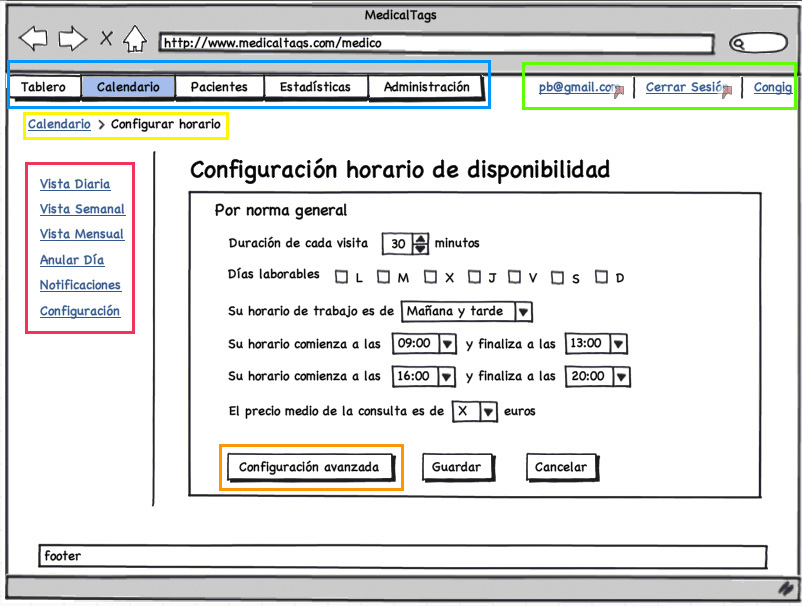
\includegraphics[width=15cm]{img/jpg/nav/medico.jpg}
			  \caption{Estructura general de los menús de navegación del médico.}
			  \label{fig:nav_medico}
			\end{figure}
			
			Si nos fijamos en la imagen (Figura \ref{fig:nav_medico}), podemos observar en azul y en verde las dos barras de navegación horizontales, en rojo la columna de navegación vertical, en amarillo la barra de navegación rápida y en naranja un vínculo de navegación individual.
			
			\textbf{Barra de navegación horizontal superior derecha (Figura \ref{fig:nav_medico_sup2}).} Siempre estará situada en la parte superior derecha de la pantalla. Si en algún momento existiera desplazamiento vertical de la página (\textit{scrolling}), la barra seguiría situada en el mismo lugar, es decir, permanecería siempre visible. Permitirá a los médicos acceder a todo lo relacionado con su configuración, cerrar la sesión actual para salir del sistema y por último ir directamente a ver su perfil.
			
			\begin{figure}[H]
			  \centering
			    
\includegraphics[width=8cm]{img/jpg/nav/medico_sup2.jpg}
			  \caption{Barra de navegación horizontal superior derecha del médico.}
			  \label{fig:nav_medico_sup2}
			\end{figure}
			
			
			\textbf{Barra de navegación horizontal superior izquierda (Figura \ref{fig:nav_medico_sup1}).} Siempre estará situada en la parte superior izquierda de la pantalla. Si en algún momento existiera desplazamiento vertical de la página (\textit{scrolling}), la barra seguiría situada en el mismo lugar, es decir, permanecería siempre visible. Esta barra permitirá a los médicos moverse por las principales secciones de navegación, que como podemos observar son:
			\begin{itemize}
				\item \textit{Tablero.} Permite al médico navegar hasta el tablero, donde se encuentran una serie de actividades usuales y resúmenes.
				\item \textit{Calendario.} Permite al médico navegar a una sección donde se encuentra todo lo relacionado con su calendario.
				\item \textit{Pacientes.} Permite al médico navegar a una sección con todo lo relacionado con sus pacientes.
				\item \textit{Estadísticas.} Permite al médico navegar hasta la sección de estadísticas.
				\item \textit{Administración.} Permite al médico navegar hasta la sección de administración, donde podrá gestionar la economía.
			\end{itemize}
			
			\fbox{\parbox{15cm}{La barra de navegación horizontal superior izquierda permite a los médicos navegar por las principales secciones (agrupamiento de funcionalidades).}}
			
			\begin{figure}[H]
			  \centering
			    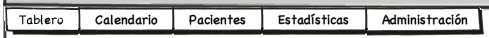
\includegraphics[width=15cm]{img/jpg/nav/medico_sup1.jpg}
			  \caption{Barra de navegación horizontal superior izquierda del paciente.}
			  \label{fig:nav_medico_sup1}
			\end{figure}
			
			\bigskip
			\bigskip
			\bigskip
			\textbf{Columna de navegación vertical izquierda (Figuras \ref{fig:nav_medico_lat1} y \ref{fig:nav_medico_lat2})}. Está situada en la parte izquierda de la pantalla, siempre por debajo de la barra de navegación superior izquierda y de la barra de navegación rápida. Realmente son varias columnas de navegación verticales, pues cada una de ellas se utiliza para navegar entre las distintas funcionalidades o subsecciones de una misma sección. A pesar de todo, todas están situadas en el mismo lugar, es decir, en la parte izquierda de la pantalla.
			
			\fbox{\parbox{15cm}{Si la barra de navegación horizontal superior izquierda permite a los médicos navegar por las principales secciones, \textbf{la columna de navegación vertical} permite navegar entre las distintas subsecciones o funcionalidades de cada sección.}}
			
			Por tanto, encontramos seis columnas de navegación verticales, cada una de ellas asociada a una sección.
			\begin{itemize}
				\item \textit{Columna de navegación vertical del Tablero (Figura \ref{fig:nav_medico_lat1})}. 
					\begin{itemize}
						\item Enlace a Ver resumen.
						\item Enlace a Próximas citas.
						\item Enlace a Últimas estadísticas.
						\item Enlace a Buscar paciente.
					\end{itemize}
				\item \textit{Columna de navegación vertical del Calendario (Figura \ref{fig:nav_medico_lat1})}.
					\begin{itemize}
						\item Enlace a Vista diaria.
						\item Enlace a Vista semanal.
						\item Enlace a Vista mensual.
						\item Enlace a Anular día.
						\item Enlace a Notificaciones.
						\item Enlace a Horario.
					\end{itemize}
				\item \textit{Columna de navegación vertical del Paciente (Figura \ref{fig:nav_medico_lat1})}.
					\begin{itemize}
						\item Enlace a Ver pacientes.
						\item Enlace a Buscar pacientes.
						\item Enlace a Ver próximos pacientes.
						\item Enlace a Ver últimos pacientes.
					\end{itemize}
				\item \textit{Columna de navegación vertical de las Estadísticas (Figura \ref{fig:nav_medico_lat2})}.
					\begin{itemize}
						\item Enlace a Estadísticas mensuales.
						\item Enlace a Estadísticas anuales.
					\end{itemize}
				\item \textit{Columna de navegación vertical de Administración (Figura \ref{fig:nav_medico_lat2})}.
					\begin{itemize}
						\item Enlace a Añadir gasto.
						\item Enlace a Añadir ingreso.
						\item Enlace a Balance global.
						\item Enlace a Historial.
					\end{itemize}
				\item \textit{Columna de navegación vertical de Configuración (Figura \ref{fig:nav_medico_lat2})}.
					\begin{itemize}
						\item Enlace a Datos.
						\item Enlace a Cuenta.
						\item Enlace a Horario.
						\item Enlace a Enviar titulación.
						\item Enlace a Notificaciones.
						\item Enlace a Motivos.
					\end{itemize}
			\end{itemize}
			
			\begin{figure}[H]
			  \centering
			    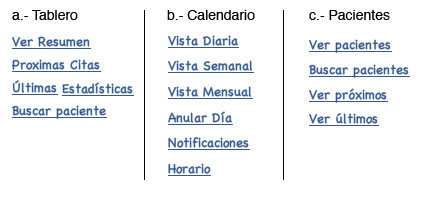
\includegraphics[width=11cm]{img/jpg/nav/medico_lat1.jpg}
			  \caption{Columnas de navegación vertical. a.- Tablero. b.- Calendario. c.- Pacientes}
			  \label{fig:nav_medico_lat1}
			\end{figure}
			
			\begin{figure}[H]
			  \centering
			    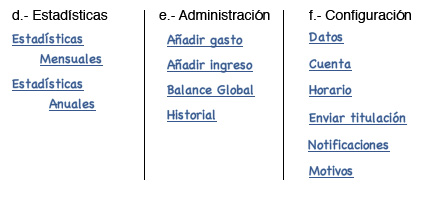
\includegraphics[width=11cm]{img/jpg/nav/medico_lat2.jpg}
			  \caption{Columnas de navegación vertical. d.- Estadísticas. e.- Administración. f.- Configuración}
			  \label{fig:nav_medico_lat2}
			\end{figure}
			
			\textbf{Barra de navegación rápida.} En todo momento podremos ver una barra de navegación rápida para saber donde nos encontramos y de donde hemos venido.
			
			\textbf{Vínculos de navegación individual.} Además de los menús de navegación que hemos mencionado y que aparecen constantemente, en diversas páginas podemos encontrar vínculos de navegación individuales. Son, principalmente:
			\begin{itemize}
				\item \textit{Ver historia clínica.} Aparece siempre que se pueda ver un paciente (en prácticamente todos los casos en la sección de Pacientes).
				\item \textit{Enviar email.} Aparece siempre que se pueda ver un paciente, igual que el caso anterior.
				\item \textit{Anular cita.} Nos lo encontramos en la vista semanal y en la diaria.
				\item \textit{Anular día.} Llama a una función que anula el día seleccionado. 
				\item \textit{Configuración avanzada.} Aparece en la configuración del horario.
				\item \textit{Adjuntar foto y adjuntar curriculum.} Enlaces habilitados en la sección de configuración para dicho fin.
				\item \textit{Modificar datos.} Para ir a los formularios correspondientes para modificar los datos.
			\end{itemize}
			
			Además, aparecen otros vínculos de uso más común con bastante frecuencia, como son:
			\begin{itemize}
				\item \textit{Guardar.} Para guardar cambios.
				\item \textit{Atrás.} Para volver a la página anterior.
				\item \textit{Cancelar.} Para no guardar los cambios realizados.
			\end{itemize}
			
			
		% paragraph menús_de_navegación_de_los_médicos (end)
		
		\paragraph{Menús de navegación de los pacientes.} % (fold)
		\label{par:nav_menus_de_navegacion_de_los_pacientes}
		
		A grosso modo, todos los menús de navegación que aparecen en las pantallas del paciente son muy similares a los de los médicos. De hecho, la estructura es la misma, y en todas las pantallas encontramos dos barras de navegación horizontales situadas siempre en la parte superior, una columna de navegación vertical (por cada sección) situada siempre en el extremo izquierdo y una barra de navegación rápida situada en la zona superior izquierda. Además, en diversas secciones también aparecen vínculos de navegación individuales.
		
		\begin{figure}[H]
		  \centering
		    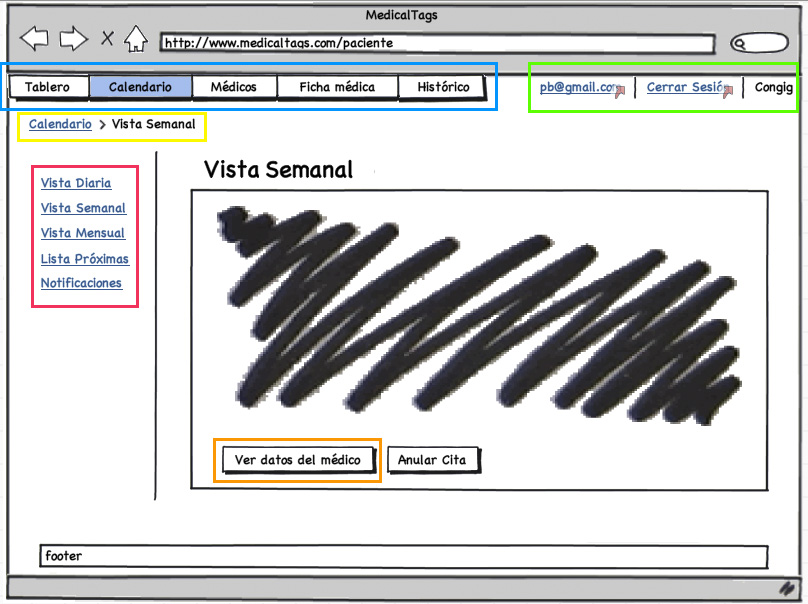
\includegraphics[width=15cm]{img/jpg/nav/paciente.jpg}
		  \caption{Estructura general de los menús de navegación del paciente.}
		  \label{fig:nav_paciente}
		\end{figure}
		
		Podemos observar en la Figura \ref{fig:nav_paciente} que en los recuadros azul y verde aparecen las dos barras de navegación horizontales, en rojo la columna de navegación vertical, en amarillo la barra de navegación rápida y en naranja un vínculo de navegación individual.
		
		\textbf{Barra de navegación horizontal superior derecha (Figura \ref{fig:nav_paciente_sup2}).} Es la misma que la del médico, por tanto, siempre estará situada en la parte superior derecha de la pantalla. Si en algún momento existiera desplazamiento vertical de la página (\textit{scrolling}), la barra seguiría situada en el mismo lugar, es decir, permanecería siempre visible. Permitirá a los pacientes acceder a todo lo relacionado con su configuración, cerrar la sesión actual para salir del sistema y por último ir directamente a ver su perfil.
		
		\begin{figure}[H]
		  \centering
		    
\includegraphics[width=8cm]{img/jpg/nav/medico_sup2.jpg}
		  \caption{Barra de navegación horizontal superior derecha del paciente.}
		  \label{fig:nav_paciente_sup2}
		\end{figure}
		
		\bigskip
		\bigskip
		\textbf{Barra de navegación horizontal superior izquierda (Figura \ref{fig:nav_medico_sup1}).} Es muy similar a la de los médicos, sin embargo, las secciones a las que permite acceder son diferentes. En cuanto a situación, como ocurría con la de los médicos, siempre estará en la parte superior izquierda de la pantalla. Si en algún momento existiera desplazamiento vertical de la página (\textit{scrolling}), la barra seguiría situada en el mismo lugar, es decir, permanecería siempre visible. Esta barra permitirá a los pacientes moverse por las principales secciones de navegación, que como podemos observar son:
		\begin{itemize}
			\item \textit{Tablero.} Permite al paciente navegar hasta el tablero, donde se encuentran una serie de actividades usuales y resúmenes.
			\item \textit{Calendario.} Permite al paciente navegar a una sección donde se encuentra todo lo relacionado con su calendario.
			\item \textit{Médicos.} Permite al paciente navegar a una sección con todo lo relacionado con los médicos.
			\item \textit{Ficha médica.} Permite al paciente navegar hasta su ficha médica.
			\item \textit{Histórico.} Permite al paciente navegar hasta la sección de su histórico, donde podrá observar cualquier acontecimiento relevante.
		\end{itemize}
		
		\fbox{\parbox{15cm}{La barra de navegación horizontal superior izquierda permite a los pacientes navegar por las principales secciones (agrupamiento de funcionalidades).}}
		
		\begin{figure}[H]
		  \centering
		    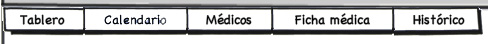
\includegraphics[width=15cm]{img/jpg/nav/paciente_sup1.jpg}
		  \caption{Barra de navegación horizontal superior izquierda de los pacientes.}
		  \label{fig:nav_paciente_sup1}
		\end{figure}
		
		\textbf{Columna de navegación vertical izquierda (Figura \ref{fig:nav_medico_lat1})}. Al igual que ocurría con los médicos, está situada en la parte izquierda de la pantalla, siempre por debajo de la barra de navegación superior izquierda y de la barra de navegación rápida. Son varias columnas de navegación verticales, pues cada una de ellas se utiliza para navegar entre las distintas funcionalidades o subsecciones de una misma sección. A pesar de todo, todas están situadas en el mismo lugar, es decir, en la parte izquierda de la pantalla.
		
		\fbox{\parbox{15cm}{Si la barra de navegación horizontal superior izquierda permite a los pacientes navegar por las principales secciones, \textbf{la columna de navegación vertical} permite navegar entre las distintas subsecciones o funcionalidades de cada sección.}}
		
		En este caso encontramos cuatro columnas de navegación verticales, cada una de ellas asociada a una sección.
		\begin{itemize}
			\item \textit{Columna de navegación vertical del Tablero (Figura \ref{fig:nav_paciente_lat1})}. 
				\begin{itemize}
					\item Enlace a Últimos resultados.
					\item Enlace a Médicos favoritos.
					\item Enlace a Añadir dato.
				\end{itemize}
			\item \textit{Columna de navegación vertical del Calendario (Figura \ref{fig:nav_paciente_lat1})}.
				\begin{itemize}
					\item Enlace a Vista diaria.
					\item Enlace a Vista semanal.
					\item Enlace a Vista mensual.
					\item Enlace a Lista de próximas citas.
					\item Enlace a Notificaciones.
				\end{itemize}
			\item \textit{Columna de navegación vertical de los Médicos (Figura \ref{fig:nav_paciente_lat1})}.
				\begin{itemize}
					\item Enlace a Buscar médicos.
					\item Enlace a Ver favoritos.
					\item Enlace a Ver próximos médicos.
					\item Enlace a Ver últimos médicos.
					\item Enlace a Ver todos mis médicos.
				\end{itemize}
			\item \textit{Columna de navegación vertical de Configuración (Figura \ref{fig:nav_paciente_lat1})}.
				\begin{itemize}
					\item Enlace a Datos.
					\item Enlace a Cuenta.
					\item Enlace a Notificaciones.
				\end{itemize}
		\end{itemize}
		
		\begin{figure}[H]
		  \centering
		    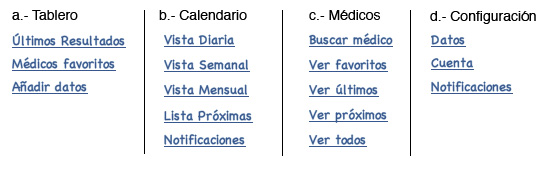
\includegraphics[width=11cm]{img/jpg/nav/paciente_lat1.jpg}
		  \caption{Columnas de navegación vertical. a.- Tablero. b.- Calendario. c.- Médicos. d.- Configuración}
		  \label{fig:nav_paciente_lat1}
		\end{figure}
		
		\textbf{Barra de navegación rápida.} En todo momento podremos ver una barra de navegación rápida para saber donde nos encontramos y de donde hemos venido, tal y como ocurría con los menús de navegación de los médicos.
		
		\textbf{Vínculos de navegación individual.} Además de los menús de navegación que hemos mencionado y que aparecen constantemente, en diversas páginas podemos encontrar vínculos de navegación individuales. Son, principalmente:
		\begin{itemize}
			\item \textit{Ver datos del médico.} Aparece siempre que se pueda ver un médico (en prácticamente todos los casos en la sección de Médicos).
			\item \textit{Enviar horarios.} Aparece siempre que se pueda ver un médico, igual que el caso anterior.
			\item \textit{Añadir a favoritos.} Como en los dos casos anteriores, es un enlace que aparece cuando tenemos localizado un médico.
			\item \textit{Anular cita.} Podemos acceder a este enlace desde la vista semanal o diaria del calendario. 
		\end{itemize}
		
		Además, aparecen otros vínculos de uso más común con bastante frecuencia, como son:
		\begin{itemize}
			\item \textit{Guardar.} Para guardar cambios.
			\item \textit{Atrás.} Para volver a la página anterior.
			\item \textit{Cancelar.} Para no guardar los cambios realizados.
		\end{itemize}
		
		% paragraph menús_de_navegación_de_los_pacientes (end)
		
		\paragraph{Menús de navegación de los administradores.} % (fold)
		\label{par:nav_menus_de_navegacion_de_los_administradores}
		
		En todas las pantallas del administrador encontramos una columna de navegación vertical situada siempre en el extremo izquierdo y una barra de navegación rápida situada en la zona superior izquierda. Además, en diversas secciones también aparecen vínculos de navegación individuales.
		
		\begin{figure}[H]
		  \centering
		    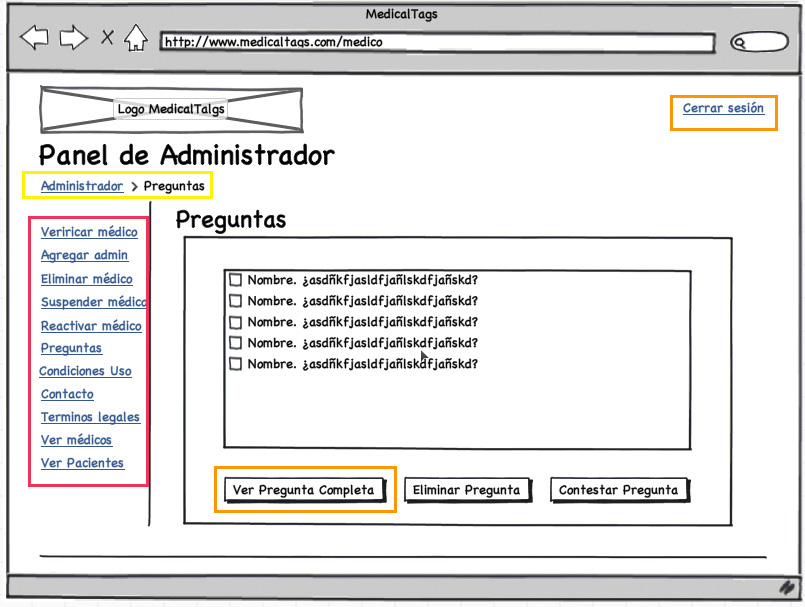
\includegraphics[width=15cm]{img/jpg/nav/administrador.jpg}
		  \caption{Estructura general de los menús de navegación del administrador.}
		  \label{fig:nav_administrador}
		\end{figure}
		
		Podemos observar en la Figura \ref{fig:nav_administrador} que en el recuadro en rojo aparece la columna de navegación vertical, en amarillo la barra de navegación rápida y en naranja los vínculos de navegación individual.
		
		\textbf{Columna de navegación vertical izquierda (Figura \ref{fig:nav_administrador_lat1})}. Está situada en la parte izquierda de la pantalla, siempre por debajo de la barra de  barra de navegación rápida. Sirve para navegar entre las distintas funcionalidades que puede llevar acabo un administrador. Los enlaces que encontramos son los siguientes (Figura \ref{fig:nav_administrador_lat1}):
		
		\begin{itemize}
			\item \textit{Verificar médico }. Lleva al administrador a la funcionalidad que le permite verificar y activar un médico.
			\item \textit{Agregar administrador.} Permite al administrador llegar a la funcionalidad de agregar un nuevo administrador.
			\item \textit{Eliminar médico.} Enlaza con la funcionalidad de eliminar médicos.
			\item \textit{Suspender médico.} Permite al administrador llegar a la funcionalidad de suspender médicos.
			\item \textit{Reactivar médico.} Lleva al administrador a la pantalla para reactivar médicos.
			\item \textit{Preguntas.} Enlaza con la sección de las preguntas.
			\item \textit{Condiciones de uso.} Enlaza con la edición de los términos legales.
			\item \textit{Contacto.} Enlaza con los datos que se desea que aparezcan en el contacto.
			\item \textit{Términos legales.} Enlaza con la edición de los términos legales.
			\item \textit{Ver médicos.} Lleva al usuario a la funcionalidad que permite buscar y ver médicos. 
			\item \textit{Ver pacientes.} Permite al administrador llegar a la funcionalidad de buscar y ver pacientes.
		\end{itemize}
		
		\begin{figure}[H]
		  \centering
		    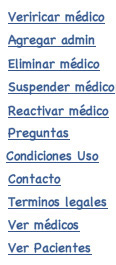
\includegraphics[width=3cm]{img/jpg/nav/administrador_lat1.jpg}
		  \caption{Columna de navegación vertical del administrador.}
		  \label{fig:nav_administrador_lat1}
		\end{figure}
		
		\textbf{Barra de navegación rápida.} En todo momento podremos ver una barra de navegación rápida para saber donde nos encontramos y de donde hemos venido, tal y como ocurría con los menús de navegación de los médicos y los pacientes.
		
		\textbf{Vínculos de navegación individual.} Los principales vínculos individuales que nos encontramos son:
		\begin{itemize}
			\item \textit{Activar médico.} Enlaza con la función habilitada para activar un médico.
			\item \textit{Eliminar médico.} Enlaza con la función habilitada para eliminar un médico.
			\item \textit{Suspender médico.} Enlaza con la función habilitada para suspender un médico.
			\item \textit{Reactivar médico.} Enlaza con la función habilitada para reactivar un médico. 
			\item \textit{Ver pregunta.} Una vez seleccionada la pregunta, nos lleva a ver su contenido íntegro.
			\item \textit{Contestar pregunta.} Una vez escrito el texto con la respuesta, enlaza con la función que se encarga de enviar el email.
			\item \textit{Eliminar pregunta.} Permite borrar una pregunta.
			\item \textit{Ver información de médico.} Una vez seleccionado el médico, nos lleva a ver su información.
			\item \textit{Ver información de paciente.} Una vez seleccionado el paciente, nos lleva a ver su información.
		\end{itemize}
		
		Además, aparecen otros vínculos de uso más común con bastante frecuencia, como son:
		\begin{itemize}
			\item \textit{Guardar.} Para guardar cambios.
			\item \textit{Atrás.} Para volver a la página anterior.
			\item \textit{Cancelar.} Para no guardar los cambios realizados.
			\item \textit{Buscar.} Cuando realizamos cualquier búsqueda, para enlazar con la función correspondiente.
		\end{itemize}
		
		
		% paragraph menús_de_navegación_de_los_administradores (end)
		
		\paragraph{Menús de navegación de las fichas médicas.} % (fold)
		\label{par:nav_menus_de_navegacion_de_las_fichas_medicas}
		
		A continuación se definen los menús de navegación de las fichas médicas, sin embargo, para llegar a la pantalla en la que aparecen, tenemos dos posibilidades: si somos médicos, accediendo a la ficha médica del paciente; si somos pacientes, accediendo a la sección de la ficha médica desde la barra de navegación superior izquierda. Por tanto, no nos interesa como llegar, sino lo que podemos hacer una vez estemos en ellas. 
		
		En términos generales, en todas las pantallas de las fichas médicas encontramos menús con pestañas horizontales, que definen las principales secciones de las fichas médicas. Estarán siempre por debajo de las barras de menús superiores que caracterizan o a médicos o a pacientes. Además, en diversas pestañas (secciones), aparecen una serie de pestañas verticales, para representar subsecciones. Por último, encontramos vínculos de navegación individuales.
		
		\begin{figure}[H]
		  \centering
		    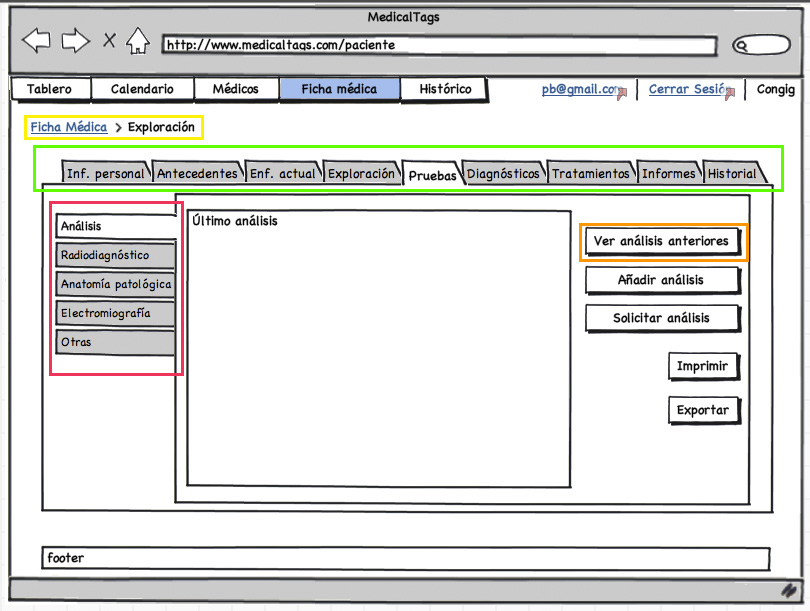
\includegraphics[width=15cm]{img/jpg/nav/fichamedica.jpg}
		  \caption{Estructura general de las fichas médicas.}
		  \label{fig:nav_ficha}
		\end{figure}
		
		Si nos fijamos en la imagen (Figura \ref{fig:nav_ficha}), podemos observar en verde las pestañas de navegación horizontales, en rojo las pestañas de navegación verticales, en amarillo la barra de navegación rápida y en naranja los vínculos de navegación individual.
		
		\textbf{Pestañas de navegación horizontal (Figura \ref{fig:nav_ficha_sup1}).} Será la cabecera de toda la información relevante a las fichas médicas. Estas pestañas permitirán a médicos y pacientes moverse por las principales secciones de las fichas médicas, que como podemos observar son:
		\begin{itemize}
			\item \textit{Información personal.} 
			\item \textit{Antecedentes.}     
			\item \textit{Enfermedad actual.}
			\item \textit{Exploración.}
			\item \textit{Pruebas.}
			\item \textit{Diagnósticos.}     
			\item \textit{Tratamientos.}
			\item \textit{Informes.}
			\item \textit{Historial.}
			\item \textit{Observaciones.}     
		\end{itemize}
		
		\fbox{\parbox{15cm}{Cada pestaña enlaza con una sección (agrupamiento de funcionalidades) relacionada con algún aspecto de la ficha médica.}}
		
		\begin{figure}[H]
		  \centering
		    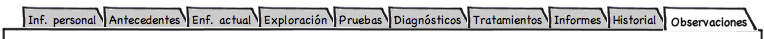
\includegraphics[width=15cm]{img/jpg/nav/fichamedica_sup.jpg}
		  \caption{Pestañas de navegación horizontales.}
		  \label{fig:nav_ficha_sup1}
		\end{figure}
		
		\textbf{Pestañas de navegación verticales izquierda (Figura \ref{fig:nav_ficha_lat1})}. Está situada en algunas pantallas en la parte izquierda, siempre dentro de alguna de las pestañas horizontales.
		
		\fbox{\parbox{15cm}{Si las pestañas de navegación horizontal permiten a los médicos y pacientes navegar por las principales secciones (agrupamiento de funcionalidades), \textbf{las pestañas de navegación vertical} permiten navegar entre las distintas subsecciones o funcionalidades de cada sección.}}
		
		Encontramos dos tipos de pestañas verticales, cada una de ellas asociada a una sección (Figura \ref{fig:nav_ficha_lat1}).
		\begin{itemize}
			\item \textit{Pestañas de navegación vertical de los Antecedentes}. 
				\begin{itemize}
					\item Enlace a Antecedentes fisiológicos.
					\item Enlace a Antecedentes familiares.
					\item Enlace a Antecedentes personales.
				\end{itemize}
			\item \textit{Pestañas de navegación vertical de las Pruebas}.
				\begin{itemize}
					\item Enlace a Análisis.
					\item Enlace a Radiodiagnóstico.
					\item Enlace a Anatomía patológica.
					\item Enlace a Electromiografía.
					\item Enlace a Otras pruebas.
				\end{itemize}
		\end{itemize}
		
		\begin{figure}[H]
		  \centering
		    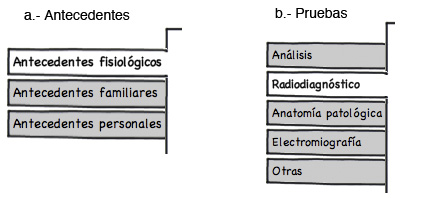
\includegraphics[width=11cm]{img/jpg/nav/fichamedica_lat.jpg}
		  \caption{Pestañas de navegación vertical. a.- Antecedentes. b.- Pruebas}
		  \label{fig:nav_ficha_lat1}
		\end{figure}
		
		
		\textbf{Barra de navegación rápida.} En todo momento podremos ver una barra de navegación rápida para saber donde nos encontramos y de donde hemos venido.
		
		\textbf{Vínculos de navegación individual.} Además de los menús de navegación que hemos mencionado y que aparecen constantemente, en diversas páginas podemos encontrar vínculos de navegación individuales. Son, principalmente:
		\begin{itemize}
			\item \textit{Ver X.} Pudiendo tomar X el valor de prueba, análisis, diagnóstico, tratamiento, informe u observación.
			\item \textit{Añadir X.}  Pudiendo tomar X el valor de prueba, análisis, diagnóstico, tratamiento, informe u observación.
			\item \textit{Solicitar X.}  Pudiendo tomar X el valor de prueba o análisis.
			\item \textit{Modificar X.} Pudiendo tomar X el valor de diagnóstico, tratamiento, informe u observación.			
		\end{itemize}
		
		Además, aparecen otros vínculos de uso más común con bastante frecuencia, como son:
		\begin{itemize}
			\item \textit{Guardar.} Para guardar cambios.
			\item \textit{Cancelar.} Para no guardar los cambios realizados.
			\item \textit{Imprimir.} Enlace a una función que permite imprimir la prueba, análisis, informe, diagnóstico, etcétera. 
			\item \textit{Exportar.} Enlace a una función que permite exportar la prueba, análisis, informe, diagnóstico, etcétera.
		\end{itemize}
		
		
		% paragraph menús_de_navegación_de_las_fichas_médicas (end)
		
		\paragraph{Menús de navegación generales.} % (fold)
		\label{par:nav_menus_de_navegacion_generales}
		
		En los menús de navegación generales existen varias pantallas. Salvo en la de registro y autentificación, que trataremos al final, el resto tienen en común que en todas encontramos una barra de navegación horizontal situada siempre en la parte superior derecha, una barra de idioma también en la parte superior derecha y una barra de navegación horizontal situada en la parte inferior. Además, podemos encontrar gran cantidad de vínculos de navegación individual
		
		\begin{figure}[H]
		  \centering
		    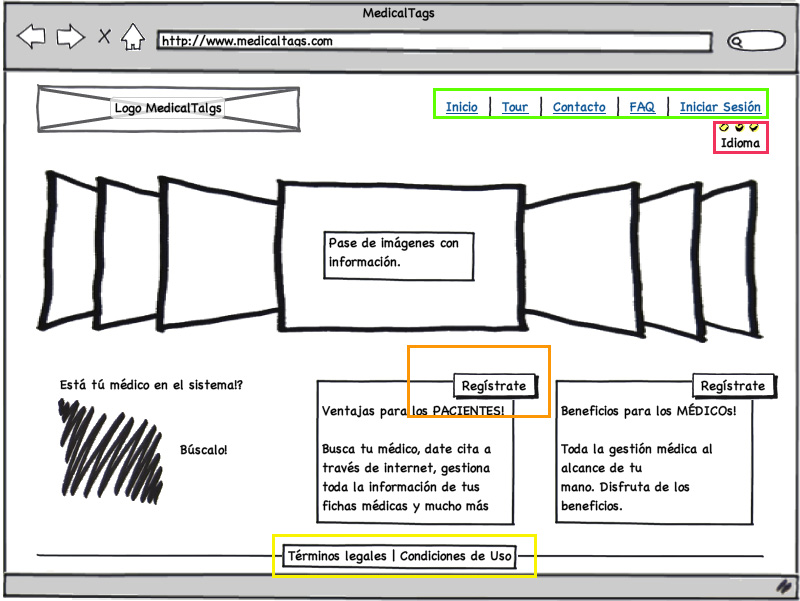
\includegraphics[width=15cm]{img/jpg/nav/general.jpg}
		  \caption{Estructura general de las páginas habilitadas para cualquier usuario.}
		  \label{fig:nav_general}
		\end{figure}
		
		Si nos fijamos en la imagen (Figura \ref{fig:nav_general}), podemos observar en verde la barra de navegación horizontal superior, en amarillo la barra de navegación horizontal inferior, en rojo la barra de idioma y en naranja un vínculo de navegación individual.
		
		\textbf{Barra de navegación horizontal superior (Figura \ref{fig:nav_general_sup}).} Siempre estará situada en la parte superior derecha de la pantalla. Si en algún momento existiera desplazamiento vertical de la página (\textit{scrolling}), en este caso la barra también se desplazaría. Permitirá a los usuarios moverse por las principales secciones de navegación, que como podemos observar son:
		\begin{itemize}
			\item \textit{Inicio.} Enlaza con el página principal.
			\item \textit{Tour.} Permite al usuario navegar a una sección donde se encuentra información algo más detallada de las funcionalidades de la aplicación.
			\item \textit{Contacto.} Enlaza con la página desde la que un usuario puede ver datos de localización y enviar un email al administrador.
			\item \textit{FAQ.} Permite al usuario navegar hasta la sección de preguntas frecuentes.
			\item \textit{Iniciar Sesión.} Enlaza con la página de inicio de sesión..
		\end{itemize}
		
		\begin{figure}[H]
		  \centering
		    
\includegraphics[width=8cm]{img/jpg/nav/general_sup.jpg}
		  \caption{Barra de navegación horizontal superior de los menús generales.}
		  \label{fig:nav_general_sup}
		\end{figure}
		
		\textbf{Barra de navegación horizontal inferior (Figura \ref{fig:nav_general_inf}).} Siempre estará situada en la parte inferior de la pantalla. Desde ella tenemos acceso a leer los términos legales y las condiciones de uso.
		
		\begin{figure}[H]
		  \centering
		    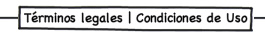
\includegraphics[width=7cm]{img/jpg/nav/general_inf.jpg}
		  \caption{Barra de navegación horizontal inferior de los menús generales.}
		  \label{fig:nav_general_inf}
		\end{figure}
		
		\textbf{Barra de idiomas}. Ofrece dos idiomas, español e inglés.
		
		\textbf{Vínculos de navegación individual.} En diversas páginas podemos encontrar vínculos de navegación individuales. La gran mayoría son:
		\begin{itemize}
			\item \textit{Inicio.}
				\begin{itemize}
					\item Buscar médico.
				\end{itemize}
			\item \textit{Tour.}
				\begin{itemize}
					\item Buscar médico.
					\item Citas \textit{online.}
					\item Ficha médica \textit{online.}
					\item Exportación de datos.
					\item Gestión de agenda \textit{online.}
					\item Gestión de pacientes \textit{online.}
					\item Gestión del centro médico \textit{online.}
					\item Notificaciones.
				\end{itemize}
			\item \textit{Contacto.}
				\begin{itemize}
					\item Enlace a twitter.
					\item Enlace a facebook.
					\item Botón enviar.
				\end{itemize}
		\end{itemize}
		
		Además, aparecen otros vínculos de uso más común con bastante frecuencia, como son:
		\begin{itemize}
			\item \textit{Registrarse como médico.} Para guardar cambios.
			\item \textit{Registrarse como paciente.} Para volver a la página anterior.
			\item \textit{Cancelar.} Para no guardar los cambios realizados.
			\item \textit{Atrás.} Para volver a la página anterior.
		\end{itemize}	
		
		% paragraph menús_de_navegación_generales (end)
		
	% subsection diseño_de_menús_de_navegación (end)

	
	
		%\begin{figure}[H]
		%  \centering
		%    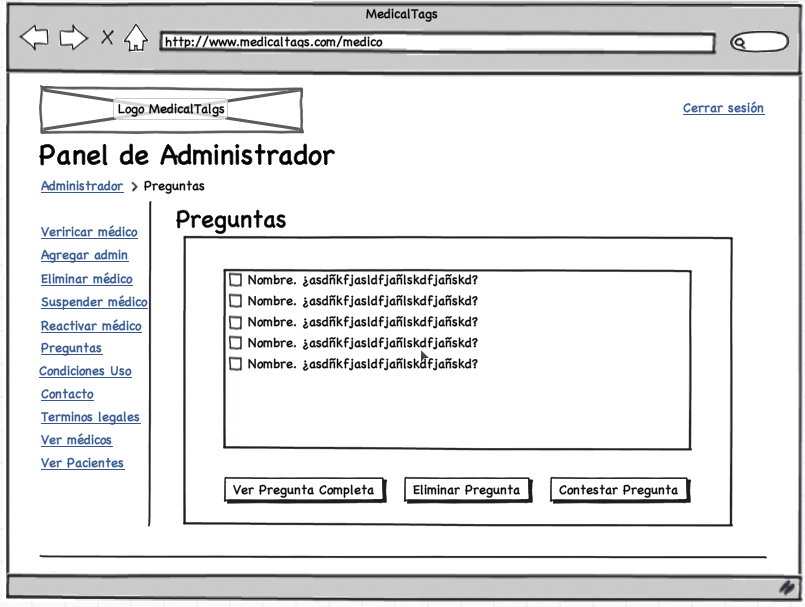
\includegraphics[width=12cm]{img/png/interfaz/99_Administrador.png}
		%  \caption{Panel de Administrador. Preguntas.}
		%  \label{fig:iu_admin_preguntas}
		%\end{figure}
	
	
		% section navegación (end)
\end{document}
% chapter diseño (end)